\documentclass[11pt,a4paper]{article}
\usepackage[utf8]{inputenc}
\usepackage{amsmath}
\usepackage{mathtools}
\usepackage{amsfonts}
\usepackage{amssymb}
\usepackage{graphicx}
\usepackage{caption}
\usepackage{subcaption}
\usepackage{comment}
\usepackage{color}
\usepackage{enumitem}
\usepackage[left=2cm,right=2cm,top=2cm,bottom=2cm]{geometry}
\usepackage{listings}
\usepackage{color}
% \usepackage[framed,numbered,autolinebreaks,useliterate]{mcode}

\setlength{\jot}{10pt}
 
\definecolor{codegreen}{rgb}{0,0.6,0}
\definecolor{codegray}{rgb}{0.5,0.5,0.5}
\definecolor{codepurple}{rgb}{0.58,0,0.82}
\definecolor{backcolour}{rgb}{0.95,0.95,0.92}
 
\lstdefinestyle{mystyle}{
    backgroundcolor=\color{backcolour},   
    commentstyle=\color{codegreen},
    keywordstyle=\color{magenta},
    numberstyle=\tiny\color{codegray},
    stringstyle=\color{codepurple},
    basicstyle=\footnotesize,
    breakatwhitespace=false,         
    breaklines=true,                 
    captionpos=b,                    
    keepspaces=true,                 
    numbers=left,                    
    numbersep=5pt,                  
    showspaces=false,                
    showstringspaces=false,
    showtabs=false,                  
    tabsize=2
}
 
\lstset{style=mystyle}
\graphicspath{ {./figures/} }
\author{Cali Greenbaum, Matthew Teta, Zane Schuessler}
\title{The Application of Linear Algebra in Netflix Algorithms}
\date{April 29 2022}

\begin{document}

\maketitle
\begin{center}
    
\includegraphics[width=0.8\textwidth]{title_img.jpeg}
\end{center}
\begin{abstract}
    In this paper we will investigate the topic of content recommendation for Netflix. Specifically, we will be investigating the algorithms Netflix uses to find movies and shows based on what the user had previously watched. The algorithms that Netflix - along with many other websites, such as Facebook, Reddit, YouTube, Instagram, and more - are based in linear algebra. Coding the software that creates the recommendations produced by these websites would not be possible without the knowledge of matrices and vectors. At the end of this paper, we will display a basic example of a linear algebra based algorithm in Python.
    \newline
    \newline
    Based on the observational nature of this paper, all members of the group were required to sufficiently research and understand the topic. As a result all three members contributed in analyzing the results and preparing the report. Matthew Teta also implemented the algorithm in python in this paper.
\end{abstract}

\pagebreak

\tableofcontents

\pagebreak

\section{Introduction} \label{sec_intro}

The application of linear algebra in user recommendations is utilized as a way for companies to engage users in their product. In other words, these algorithms entice us to continuously consume product. In addition to keeping viewers, or website users, from logging off and doing something else, companies will utilize their findings by collecting data. With these algorithms, Netflix and other websites with the same features have the ability to make connections between the type of content consumed and a person's location, ethnicity, income, age, among other data points that they may have access to (think: when you post on Instagram and tag your location, when you give your address to Netflix for billing, when you put your birthday into Facebook, etc.).

In order to fully understand how linear algebra is used for these algorithms, the reader of this paper should be knowledgeable of matrices, including what they look like and their associated properties, vectors and how they can interact with matrices, and the concept of data analysis. In addition to basic knowledge of linear algebra and data analysis, prior research on the ideas of back propagation and gradient descent will improve the reader's grasp of how the algorithm works.

In the Examples and Numerical Results section of this paper we demonstrate an example of the functionality of this algorithm in code. We have downloaded some movie data from the official Netflix data bank in order to prove the concepts described in the paper.



\section{Mathematical Formulation}

Netflix and other websites that model consumer algorithms need places to store the data that they collect. The collected data is placed into vectors, then into matrices, and then stored and tied to your unique account ID.

Consider all TV shows that are available to watch in Netflix. TV shows with similar genres are represented by similar numerical values, for example, Love is Blind and The Ultimatum may be represented by 20 and 21, respectively.

Let the following matrix, Matrix A, represent all of the dating shows a user may have watched in a certain period of time, for example, 6 months. These data points for all dating shows are roughly around the number 20. Matrix A may look something like:

\begin{align*}
    A = \begin{bmatrix}
            21 & 22 & 23 \\
            20 & 25 & 22
        \end{bmatrix}
\end{align*}

Let Matrix B represent horror shows, most of which are represented by the number 10:

\begin{align*}
    B = \begin{bmatrix}
            11 & 10 & 14 \\
            12 & 12 & 13
        \end{bmatrix}
\end{align*}

Finally, let Matrix C represent cooking shows, most of which are represented by the number 30.

\begin{align*}
    C = \begin{bmatrix}
            30 & 32 & 33 \\
            35 & 31 & 34
        \end{bmatrix}
\end{align*}

The matrices A, B, and C are the principal/typical components of the set of movies offered. This means that each matrix represents a specific aspect underlying the data (in this case, the aspects are genres). Utilizing matrix addition and singular value decomposition (SVD), Netflix can determine what shows to suggest to any given user. If the user clicks on dating shows more often than horror shows, but clicks on cooking shows more than horror shows, Netflix's formula for its algorithm may look something like:

\begin{equation}
    AM = A + 0.5B + .001C
\end{equation}
\hfill

\noindent With AM representing the final "Algorithm Matrix". The result of this matrix addition and multiplication is as follows:

\begin{equation}
    AM = \begin{bmatrix}
        21 & 22 & 23 \\
        20 & 25 & 22
    \end{bmatrix} + .5*\begin{bmatrix}
        11 & 10 & 14 \\
        12 & 12 & 13
    \end{bmatrix} + .001\begin{bmatrix}
        30 & 32 & 33 \\
        35 & 31 & 34
    \end{bmatrix}
\end{equation}
\hfill
\begin{equation}
    AM = \begin{bmatrix}
        26.53  & 27.032 & 30.033 \\
        26.035 & 31.031 & 28.534
    \end{bmatrix}
\end{equation}

As shown in the final algorithm matrix, Netflix now knows what types of shows to suggest. Four of those values are in the 20s, suggesting to Netflix that this user likes dating shows. There are two values in the 30s, suggesting that this user may also like horror shows. The more that the user clicks on cooking shows as opposed to horror and dating, the values in this matrix will change. Starting from a completed AM matrix, these calculations can be done in reverse order using principal component analysis (PCA) to find the typical components, A, B, and C.

This strategy works well for forming AM when the principal components are known and the user has submitted a rating for every show. The question now, is how to create AM when the user has not watched all the shows. Because the matrix AM is now sparse, the SVD of AM is now undefined.

Assume a $u \times t$ rating matrix $R$ of a set of movies is dense (every user has submitted a rating for every title on Netflix). The PCA of R and the transpose of R will give typical users and movies as vectors that can then be formed into a set of matrices U and M. The SVD of R can be represented by,
\begin{align*}
    R = M\Sigma U^T \\
    R = M U^T
\end{align*}

With $U$ being the $u \times f$ matrix of typical users and $M$ the $t \times f$ matrix of typical movies. Importantly, the common dimension $f$ is the number of latent factors that describes the users and titles. This process reduces the size of the data significantly, and it allows us to represent our original matrix $R$ with two much smaller matrices. $\Sigma$ can be neglected as it is just a diagonal matrix to scale the rows and columns of the U and M matrices. Considering the rating of user \textit{u} for movie \textit{i} gives the form,
\begin{align*}
    \begin{bmatrix}
        r_{ui}
    \end{bmatrix}
    =
    \begin{bmatrix}
        - p_\textit{u} -
    \end{bmatrix}
    \begin{bmatrix}
        |            \\
        q_\textit{i} \\
        |            \\
    \end{bmatrix}
    \\
    r_{ui} = p_u \cdot q_i
\end{align*}

Now, in the Netflix data case, R is no longer dense. It is not possible to use traditional SVD methods, because it is not even possible to pull out the eigenvalues from the original matrix. Furthermore, the (sparse) matrix is about 99\% empty. However impossible it may seem to generate so many remaining values from the limited amount of data known, there is a method which has proven to be very successful. Since the minimization is only depends on the known values of the $R$ matrix, the resulting factorization can be used to extrapolate estimates for the unknown values later on. Simon Funk developed the minimization function used in the algorithm.
\begin{equation}
    \min_{p_u,q_i} \sum_{r_{ui} \in R} (r_{ui} - p_u \cdot q_i)^2
\end{equation}

Finding exact values of $p_u$ and $q_i$ that minimize the sum is a very hard process since it cannot be solved directly, and computational estimates are inefficient on large data. Instead we will approximate the values using the stochastic gradient descent (SGD) technique. This technique repeatedly computes the partial derivatives of the the error function in order to adjust the values in the solution matrices and trend toward (a) minimum. The algorithm uses back propagation to find gradients needed for SGD. Because the minimization can be written as a function of $p_u$ and $q_i$, that is,
\begin{equation}
    f(p_u, q_i) = \sum_{r_{ui} \in R} (r_{ui} - p_u \cdot q_i)^2 = f_{ui}(p_u, q_i)
\end{equation}
The SGD procedure requires the partial derivative of $f$ with respect to both $p_u$ and $q_i$ be taken for all known values of $r_{ui}$.
Starting out by randomly initializing $p_u$ and $q_i$, we take the partial of a specific known $r_{ui}$ value and then update $p_u$ and $q_i$ according to the following rule,

\begin{align*}
    p_u \leftarrow p_u + \alpha \cdot q_i(r_{ui} - p_u \cdot q_i) \\
    q_i \leftarrow q_i + \alpha \cdot p_u(r_{ui} - p_u \cdot q_i)
\end{align*}

The method is applied for all known values, $r_{ui}$, and repeated for a number of epochs. The learning rate, $\alpha$, is a constant that determines how large the iterations steps are. The smaller the learning rate, the more epochs are necessary for reaching a minimum. A smaller learning rate also provides the benefit of following the surface of the minimization function more closely, so high frequency details won't be skipped over. The goal is to reach the absolute minimum, not a local minimum. This can be tough with this technique, since it is highly dependent on the starting points for $p$ and $q$, and fluctuations in the terrain will lead to many false / local minimums. The model can be trained multiple times until the best solution is found. Once all the $p_u$ and $q_i$ vectors have been computed to satisfaction, a completed rating matrix R with approximate rating values can be created from the simple formula,
\begin{align*}
    \hat{r}_{ui} & \approx p_u \cdot q_i \\
    R            & \approx P Q
\end{align*}

We denote $\hat{r}_{ui}$ with a hat because the values are just estimates and not exact. With this algorithm, the idea of approximating values based on known data can be used more generally outside of just Netflix's recommendations.
\section{Examples and Numerical Results}

% \subsection{Data Import and Analysis}

In order to fully understand the way Netflix handles and reads data for their algorithm, we decided to create a similar algorithm by importing a data set containing 100,480,507 unique user ratings. The data is provided in four ~500Mb files each containing sections for movie IDs and rows containing a user ID, rating, and date of rating. For example,

\begin{verbatim}
189:
1943087,5,2001-10-20
306466,4,2001-09-21
1966165,5,2004-02-10
\end{verbatim}

It was necessary to write a custom parser that reads in the data files line by line and pulls out the columns. The data is then formatted into a data frame for ease of use with the Plotly graphing library. In addition, since the user IDs are randomly assigned, we had to map them to array indices to reduce the size of the p and q matrices later.
\newpage
\begin{lstlisting}[language=Python]
import numpy as np
import pandas as pd
import plotly.express as px
from typing import List
from datetime import datetime

def load_data(filepaths: List[str], import_date=False):
    '''Generate a list of all data entries from the given list of file paths
    '''
    data = dict(
        item_id=[],
        user_id=[],
        item_index=[],
        user_index=[],
        rating=[]
    )
    if import_date:
        data['date'] = []
    user_id_map = {}
    item_id_map = {}
    item_id = 0
    for fname in filepaths:
        with open(fname, 'r') as input_file:
            for line in input_file:
                if line[-2] == ':':
                    # Set item_id when we encouter a new section of the data
                    item_id = int(line[:-2])
                else:
                    # Line has a user rating in it, capture the values and store in array
                    [user_id, rating, date] = line.split(',')
                    user_id = int(user_id)
                    if import_date:
                        date = datetime.strptime(date.rstrip(), '%Y-%m-%d')

                    if (not item_id in item_id_map):
                        item_id_map[item_id] = len(item_id_map)
                    if (not user_id in user_id_map):
                        user_id_map[user_id] = len(user_id_map)

                    rating = float(rating)

                    data['item_id'].append(item_id)
                    data['user_id'].append(user_id)
                    data['item_index'].append(item_id_map[item_id])
                    data['user_index'].append(user_id_map[user_id])
                    data['rating'].append(rating)
                    if import_date:
                        data['date'].append(date)
    data = pd.DataFrame(data)
    return (dict(
        n_items=len(item_id_map),
        n_users=len(user_id_map),
        data=data
    ),
    user_id_map,
    item_id_map)
\end{lstlisting}

\newpage

To make it more manageable, the data needed to be pared into a smaller size so that it would process more quickly for testing and development purposes. While this may affect the overall results of the code, it is not possible to run the full amount of data on a personal computer. The following plot provides an rough the size of the data set of the first 100 ratings for each movie ID. There is an interactive version of the plot that can be seen by cloning the Jupyter Notebook from my GitHub.

\begin{figure}[h]
    \centering
    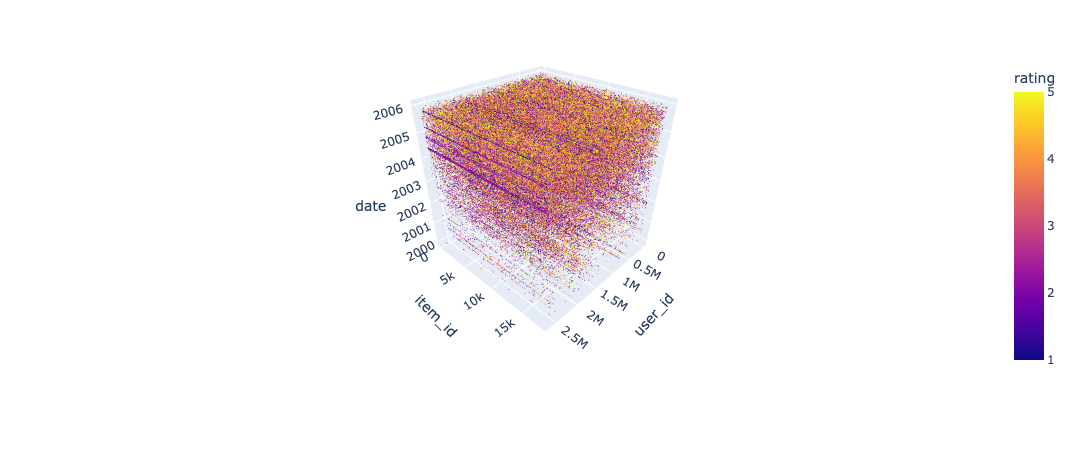
\includegraphics[width=\textwidth]{3d_scatter_home.png}
\end{figure}

This plot is useful to show that the user id field is normally distributed, and the number of Netflix users increased dramatically around 2005.

\begin{figure}[h]
    \centering
    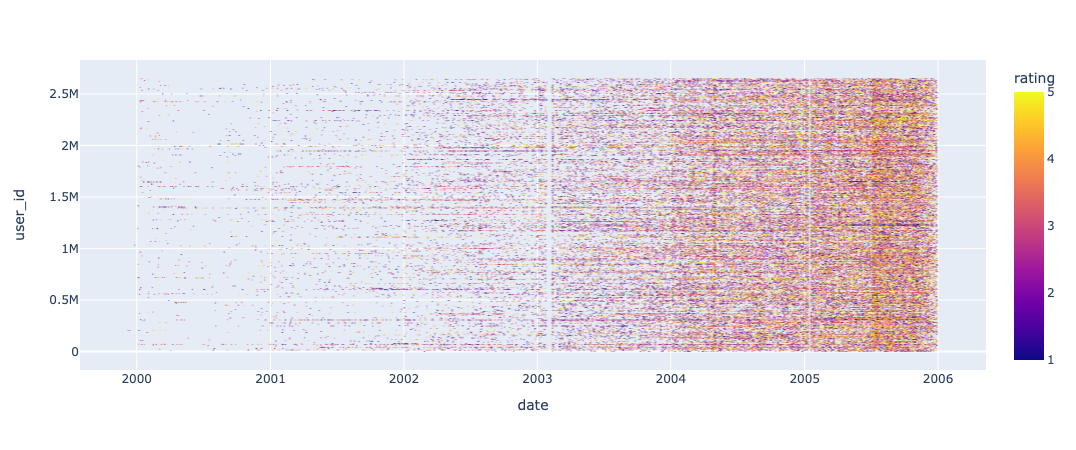
\includegraphics[width=\textwidth]{scatter_date_vs_user_id.png}
\end{figure}

\newpage
Once the data is imported into python, we can feed it into the gradient descent algorithm,

\begin{lstlisting}[language=Python]
def gradient_descent(dataset, n_factors=10, learning_rate=0.01, n_epochs=10):
    '''Learn the reduced dimension matricies p and q from the data points in the data array
    '''
    # initialize p and q randomly
    # p is user matrix and q is the movie matrix
    p = np.random.normal(0, .1, (dataset['n_users'], n_factors))
    q = np.random.normal(0, .1, (dataset['n_items'], n_factors))

    data = dataset['data']

    # optimize
    for _ in range(n_epochs):
        for ind in data.index:
            p_ind = data['user_index'][ind]
            q_ind = data['item_index'][ind]
            rating = data['rating'][ind]
            # Pull values onto stack for efficiency
            # Calculate gradient descent error
            err = rating - np.dot(p[p_ind], q[q_ind])
            adj = err * learning_rate
            # Apply descent correction
            p[p_ind] += adj * q[q_ind]
            q[q_ind] += adj * p[p_ind]

    # return the matricies
    return (p, q)


\end{lstlisting}

This training process takes the longest time out of all of the computations. At first, we attempted to run the entire data set, but this was still not completed after 40 hours, so it was necessary to end the processing. Interestingly, it would be possible to save the $p$ and $q$ matrices to use them as the starting point for training when new data becomes available. It would also be possible to modify the algorithm to only use new ratings to update the existing prediction model. Optimizing in this way causes the overall speed of the algorithm to improve significantly. In fact, it would be very fast to update the model instantly any time a rating is made on the Netflix platform.
With the trained $p$ and $q$ models in memory, it becomes time to make some rating predictions! We can use the following functions to generate recommendations.

\begin{lstlisting}[language=Python]
def estimate(user_factors, item_factors, user_id, item_id, user_id_map, item_id_map):
    return np.dot(user_factors[user_id_map[user_id]], item_factors[item_id_map[item_id]])

def estimate_with_index(user_factors, item_factors, user_index, item_index):
    return np.dot(user_factors[user_index], item_factors[item_index])
\end{lstlisting}

There are two versions of the function since we remapped the indices of the user IDs and title IDs. By taking a dot product, the data processing becomes a very fast process and a single rating can be generated in milliseconds even in Python. We estimated the predictions from the model for all of the known ratings and put them into a data frame consistent with the first one,

\begin{lstlisting}[language=Python]
# Generate data frame identical to the actual values but with the predictions
pred_ratings = np.zeros(len(dataset['data']['rating']))
for ind in dataset['data'].index:
    user_index = dataset['data']['user_index'][ind]
    item_index = dataset['data']['item_index'][ind]
    pred_ratings[ind-1] = estimate_with_index(user_factors, movie_factors, user_index, item_index)
predictionset = pd.DataFrame(dict(
    rating=pred_ratings,
    user_index=dataset['data']['user_index'],
    item_index=dataset['data']['item_index'],
    user_id=dataset['data']['user_id'],
    item_id=dataset['data']['item_id']
))

err = dataset['data']['rating'] - predictionset['rating']
df2 = pd.DataFrame(dict(err=err, user_index=predictionset['user_index'], item_index=predictionset['item_index']))
\end{lstlisting}

In order to analyze the success of the matrix factorization and gradient decent minimization, we generated a number of error measurements and summary statistics using this error data frame and the \texttt{df2} data frame. Using Plotly, we generated this histogram which shows the distribution of the error in the model.

\begin{figure}[h]
    \centering
    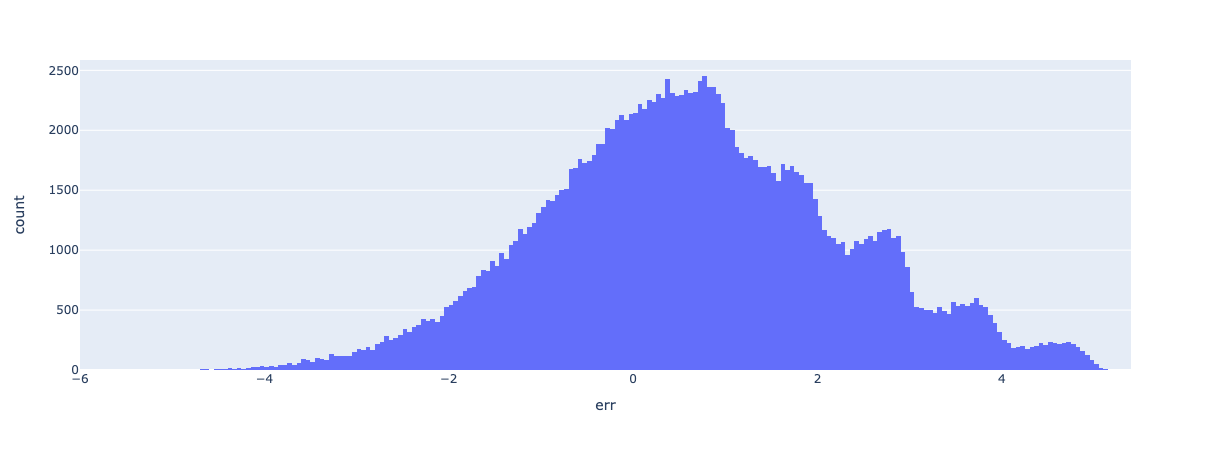
\includegraphics[width=\textwidth]{histogram_err.png}
    \caption{$\mu=0.667$, $\sigma=1.62$}
\end{figure}

Error exists in our data since we were not able to include the entire data set. The subset of data that we used is only about 0.2\% of the entire Netflix data set. In addition, in order to even more accurately evaluate the error, it would be necessary to split the data set into a 'training' and an 'evaluation' set. This way, the error is measured by the success of the predictions. This was challenging to do without selecting the subset of data more carefully to contain a subset of the users and titles. This is because a prediction has no meaning if the user does not have any ratings at all, which is highly likely in the small data set that we used. For this reason, we chose to measure the error only based on the points used to train the model.

% \begin{lstlisting}[language=Python]

% \end{lstlisting}

\section{Discussion and Conclusion}

It is interesting to consider how the rating algorithm can be modified to include other factors. For example, cursor hover time, time spent reading a caption, time spent watching, number of episodes watched, common cast between titles, title budget, director, search terms, etc. There is plent more data collected by these social media platforms that can be utilized to improve user recommendations.

Also, there should be more criteria used to filter out the data that is fed into the rating training algorithm. Bad data can ruin the utility of a model, and there are also malicious actors on the internet which can lead to data which should not be considered. It would be best to filter out preliminary data from users who haven't rated more than a few titles or who have rated titles that they haven't actually watched. Also, since the algorithm influences the titles that people watch and then rate, there is a positive feedback that can occur where the recommendations are reinforced by the effect of recommending titles to users. It is almost like Netflix's algorithm is patting itself on the back. If a user decides to watch a recommended film, the algorithm will just enforce that specific film's rating: this can hurt the user's watching experience as the algorithm will be less likely to recommend new movies. Netflix has accounted for this somewhat by putting a list of newly released films at the top of the homepage. Some strategies that I imagine for minimizing this effect is to either change the weight of ratings that were a direct result of common recommendations or to throw in random titles that cause a user to be shown more options.

Also, this algorithm can be easily translated to other data sets. You could use this for book, product, advertisement, news article, or food recommendations: in layman's terms, anything consumable can be modelled. Because this algorithm is so general and highly applicable, it would be worth doing more research on similar topics. Understanding how socioeconomic biases play into the content that gets recommended to certain users might lead us to a better understanding of our societies and become more introspective and calculating about what we consume. Also, this data set is relatively small compared to the amount of data that content recommendation companies have access to, so it would be important to invest in making these run as efficiently as possible.



Learning about SVD, PCR, Gradient Descent, and Back Propagation has lead to some important insights into how modern content delivery services operate. As a consumer of media in the digital age, you must ask yourself, "What are the implications of these algorithms?" It may be that you don't want to be influenced by the mass effect of trends in human interests, or maybe you embrace it and guide the algorithm intentionally. Whatever you choose, it is interesting to understand how this works, and the scale of data that it is applied to. Personally, I'd like to imagine that the overall effect of these systems on the population of the world is positive, but there are examples in the past of similar algorithms being used with malicious intent to cause harm and alter the natural path of history.



\newpage
\begin{thebibliography}{widest entry}
    \bibitem{label1} Nicolas Hug. Understanding Matrix Factorization for Recommendation (Part 1) - Preliminary Insights on PCA. 14 June 2017 %http://nicolas-hug.com/blog/matrix_facto_1. 

    \bibitem{label2}Pajkovic, Niko. “Algorithms.” Sage Journals %https://journals.sagepub.com/doi/full/10.1177/13548565211014464. 

    \bibitem{label3}“Matrices, Music, and Netflix Recommendations.” UC Berkeley. %https://math.berkeley.edu/~sander/fall2016decal/reading10.pdf

    \bibitem{label4} The Netflix Prize and Singular Value Decomposition.” CS-301, New Jersey Institute of Technology %https://pantelis.github.io/cs301/docs/common/lectures/recommenders/netflix/.  

    \bibitem{label5} Chong, David. “Deep Dive into Netflix's Recommender System.” Medium, Towards Data Science, 24 Sept. 2021 %https://towardsdatascience.com/deep-dive-into-netflixs-recommender-system-341806ae3b48. 

    \bibitem{label6} Jiri Stodulka. “Collaborative Filtering: Matrix Factorization Recommender System.” Jiri Stodulka, 20 Oct. 2021 %https://www.jiristodulka.com/post/recsys_cf/. 

\end{thebibliography}

\end{document}